\section{Evaluation on ViSTR-Bench}

\begin{table}[!t]
    \centering
    \caption{
        \textbf{Main results on ViSTR-Bench.} 
        We report accuracy (\%) across 12 subtasks grouped into four reasoning dimensions.
        The suffix \emph{-thinking} indicates that the model is evaluated with its built-in thinking mode enabled.
        \emph{Avg.} denotes the overall accuracy averaged over all question-answer pairs, and \emph{Rank} denotes the ranking within each model category.
        The best and second-best results within each model group are highlighted with \bestcap{} and \secondcap{}, respectively.
    }
    \label{tab:main_results}

    \resizebox{\textwidth}{!}{
    \begin{tabular}{l c c cc cc ccccc ccc}
        \toprule
        \multirow{2}{*}{\textbf{Method}} 
        & \multirow{2}{*}{\textbf{Rank}} 
        & \multirow{2}{*}{\textbf{Avg.}} 
        & \multicolumn{2}{c}{\textbf{Motion Perc.}} 
        & \multicolumn{2}{c}{\textbf{Spat. Rela.}} 
        & \multicolumn{5}{c}{\textbf{Outc. Pred.}}  
        & \multicolumn{3}{c}{\textbf{Phys. Dyna.}} \\
        \cmidrule(lr){4-5} \cmidrule(lr){6-7} \cmidrule(lr){8-12} \cmidrule(lr){13-15}
        & & 
        & \makecell{Vehi.\\Move.} & \makecell{Rela.\\Velo.} 
        & \makecell{Ego\\Motion} & \makecell{Pass.\\Feas.} 
        & Bask. & Soccer & Golf & Bill. & Swim.
        & Jenga & Mikado & Knot \\
        \midrule

        \rowcolor{groupbg}
        \multicolumn{15}{l}{\textbf{Baseline}} \\
        Chance Level (Random) & - & 50.0 & 50.0 & 50.0 & 50.0 & 50.0 & 50.0 & 50.0 & 50.0 & 50.0 & 50.0 & 50.0 & 50.0 & 50.0 \\
        Chance Level (Frequency) & - & 57.2 & 64.3 & 59.5 & 53.4 & 65.5 & 57.3 & 52.5 & 54.7 & 53.3 & 50.0 & 65.0 & 54.2 & 58.6 \\
        \midrule

        \rowcolor{groupbg}
        \multicolumn{15}{l}{\textbf{Proprietary General MLLMs}} \\
        GPT-5.4 & 9 & 54.9 & 66.1 & 67.9 & 63.4 & 67.3 & 42.7 & 53.2 & 45.3 & 52.0 & 51.4 & 46.2 & 45.8 & 69.0 \\
        GPT-5.4-thinking & 3 & 59.0 & 57.1 & \second{75.0} & \best{75.6} & 58.2 & 46.8 & 51.3 & \second{54.7} & \best{58.7} & 50.0 & \best{67.5} & 47.0 & \second{72.4} \\
        Gemini-3-Flash-Preview & 17 & 50.0 & 35.7 & 44.0 & 55.7 & 63.6 & 44.4 & 54.4 & 49.1 & 53.3 & \second{59.7} & 44.4 & 50.6 & 62.1 \\
        Gemini-3.1-Flash-Lite-Preview & 13 & 52.4 & 45.5 & 50.0 & 62.6 & 63.6 & 53.2 & 46.8 & 49.1 & 36.0 & \second{59.7} & 60.7 & 44.6 & 65.5 \\
        Gemini-3.1-Pro-Preview & 11 & 53.6 & 45.5 & 52.4 & \second{72.5} & 65.5 & \best{56.5} & 50.0 & 43.4 & 54.7 & 50.0 & 42.7 & 47.0 & \best{75.9} \\
        Claude-Sonnet-4.6 & 16 & 52.0 & \second{67.9} & 40.5 & 64.9 & 52.7 & 54.8 & 55.1 & 50.9 & 48.0 & 50.0 & 34.2 & 38.6 & 62.1 \\
        Claude-Sonnet-4.6-thinking & 8 & 55.4 & 67.0 & 40.5 & 66.4 & 52.7 & 51.6 & \second{62.0} & \best{58.5} & 52.0 & 51.4 & 48.7 & 44.6 & 62.1 \\
        Claude-Opus-4.6 & 4 & 57.0 & 65.2 & 45.2 & 64.1 & \best{70.9} & 49.2 & \best{63.3} & 50.9 & 40.0 & 50.0 & \second{65.8} & 44.6 & \second{72.4} \\
        Claude-Opus-4.6-thinking & 6 & 56.1 & 65.2 & 40.5 & 71.8 & 67.3 & 44.4 & 56.3 & 52.8 & 46.7 & 50.0 & 65.0 & 48.2 & 55.2 \\
        Seed-2.0-Lite & 7 & 56.0 & 64.3 & 60.7 & 51.1 & 63.6 & 52.4 & 55.7 & 49.1 & 49.3 & 48.6 & 65.0 & \second{55.4} & 48.3 \\
        Seed-2.0-Lite-thinking & \second{2} & \second{59.7} & \best{68.8} & 67.9 & 66.4 & 65.5 & 49.2 & 61.4 & \best{58.5} & 48.0 & 51.4 & 65.0 & 51.8 & 51.7 \\
        Seed-2.0-Pro & 5 & 56.6 & 57.1 & 67.9 & 58.0 & \best{70.9} & 52.4 & 51.3 & 47.2 & \best{58.7} & 55.6 & 63.2 & 48.2 & 48.3 \\
        Seed-2.0-Pro-thinking & \best{1} & \best{59.8} & 63.4 & \best{81.0} & 67.9 & \second{69.1} & \second{55.6} & 53.2 & 49.1 & 54.7 & \best{66.7} & 57.3 & 45.8 & 51.7 \\
        MiMo-V2-Omni & 14 & 52.1 & 64.3 & 51.2 & 58.8 & 58.2 & 45.2 & 43.7 & 41.5 & 52.0 & 43.1 & 63.2 & 44.6 & 58.6 \\
        MiMo-V2-Omni-thinking & 10 & 54.1 & 55.4 & 45.2 & 63.4 & \best{70.9} & 44.4 & 55.1 & 43.4 & 49.3 & 48.6 & 58.1 & \best{56.6} & 58.6 \\
        MiMo-V2.5 & 15 & 52.0 & 59.8 & 40.5 & 64.9 & 50.9 & 42.7 & 55.7 & 37.7 & \second{56.0} & 52.8 & 51.3 & 42.2 & 62.1 \\
        MiMo-V2.5-thinking & 12 & 52.5 & 51.8 & 38.1 & 58.0 & 63.6 & 50.8 & 53.8 & 35.8 & 50.7 & 51.4 & 60.7 & 53.0 & 55.2 \\
        \midrule

        \rowcolor{groupbg}
        \multicolumn{15}{l}{\textbf{Open-source General MLLMs}} \\
        LLaVA-OneVision-1.5-4B & 14 & 47.8 & 60.7 & 36.9 & 52.7 & 65.5 & 42.7 & 47.5 & 54.7 & 46.7 & 50.0 & 35.0 & 45.8 & 41.4 \\
        LLaVA-OneVision-1.5-8B & 11 & 48.9 & \second{63.4} & 40.5 & 53.4 & 65.5 & 41.9 & 47.5 & 50.9 & 48.0 & 50.0 & 38.5 & 45.8 & 51.7 \\
        Qwen3.5-27B-thinking & \best{1} & \best{55.1} & 60.7 & 50.0 & 62.6 & 65.5 & \best{59.7} & \best{55.1} & 49.1 & 49.3 & \second{58.3} & 47.9 & 44.6 & 51.7 \\
        Qwen3.5-35B-A3B-thinking & 13 & 48.7 & 46.4 & 45.2 & 58.0 & 63.6 & \second{48.4} & 50.6 & 35.8 & 52.0 & 40.3 & 41.0 & 48.2 & 55.2 \\
        Qwen3.5-122B-A10B-thinking & 5 & 53.0 & 53.6 & 50.0 & 61.8 & 67.3 & \second{48.4} & 50.0 & 39.6 & \best{56.0} & 43.1 & \second{55.6} & 48.2 & \best{72.4} \\
        Qwen3.5-397B-A17B-thinking & 3 & 54.3 & 57.1 & \second{57.1} & \second{65.6} & 63.6 & \best{59.7} & 51.3 & 43.4 & 48.0 & 45.8 & 52.1 & 38.6 & \second{69.0} \\
        InternVL3.5-8B & 7 & 50.5 & 57.1 & \second{57.1} & 64.9 & \best{70.9} & 43.5 & 47.5 & 39.6 & 53.3 & 48.6 & 35.0 & 45.8 & 41.4 \\
        InternVL3.5-14B & 8 & 50.0 & 50.0 & \best{59.5} & 53.4 & 65.5 & 42.7 & 47.5 & 45.3 & 52.0 & \best{62.5} & 39.3 & 49.4 & 41.4 \\
        InternVL3.5-38B & \second{2} & \second{54.5} & 49.1 & 47.6 & 60.3 & 65.5 & 46.8 & \second{52.5} & \second{56.6} & \second{54.7} & 52.8 & \best{65.0} & \second{50.6} & 62.1 \\
        InternVL3.5-30B-A3B & 9 & 49.6 & 51.8 & \best{59.5} & 58.0 & 65.5 & 42.7 & 46.8 & 41.5 & 40.0 & 50.0 & 41.9 & \best{55.4} & 41.4 \\
        InternVL3.5-241B-A28B & 4 & 54.1 & \best{65.2} & 46.4 & \best{66.4} & \second{69.1} & 45.2 & 46.8 & 49.1 & 53.3 & 47.2 & \second{55.6} & 49.4 & 62.1 \\
        Intern-S1-thinking & 6 & 50.8 & 48.2 & \second{57.1} & 60.3 & 58.2 & \second{48.4} & 47.5 & 35.8 & \best{56.0} & 48.6 & 47.9 & 45.8 & 58.6 \\
        Intern-S1-Pro-thinking & 10 & 49.2 & 53.6 & 40.5 & 63.4 & 56.4 & 41.9 & 47.5 & \best{58.5} & 45.3 & 41.7 & 48.7 & 42.2 & 55.2 \\
        GLM-4.6V-thinking & 12 & 48.9 & 58.0 & 41.7 & 61.8 & 52.7 & 42.7 & 47.5 & 39.6 & 46.7 & 52.8 & 35.9 & 49.4 & 65.5 \\
        \midrule

        \rowcolor{groupbg}
        \multicolumn{15}{l}{\textbf{Specialized Spatial MLLMs}} \\
        SpaceR-SFT-7B & \second{2} & \second{50.7} & 46.4 & 60.7 & \best{64.9} & \second{65.5} & 42.7 & \best{51.9} & 49.1 & 50.7 & 40.3 & 35.0 & 53.0 & 58.6 \\
        VG-LLM-4B & 8 & 46.8 & 44.6 & 45.2 & 42.0 & \second{65.5} & 42.7 & 47.5 & \second{56.6} & \second{52.0} & 44.4 & 35.0 & 54.2 & 58.6 \\
        VG-LLM-8B & 10 & 45.3 & 36.6 & 39.3 & 38.2 & \second{65.5} & \best{46.0} & 48.7 & \second{56.6} & \best{53.3} & \second{50.0} & 35.0 & 45.8 & 55.2 \\
        Spatial-MLLM-135K-4B & 9 & 45.7 & 42.0 & 47.6 & 55.7 & 34.5 & 41.9 & 46.2 & 50.9 & 46.7 & \second{50.0} & 35.0 & 47.0 & 62.1 \\
        Spatial-MLLM-820K-4B & 3 & 50.5 & \best{64.3} & \second{63.1} & 45.8 & 58.2 & 42.7 & 47.5 & 54.7 & 46.7 & \second{50.0} & 35.0 & \best{57.8} & 62.1 \\
        SpatialLadder-3B & 7 & 48.2 & 52.7 & \best{67.9} & 38.9 & \best{67.3} & 43.5 & 44.3 & 45.3 & 45.3 & \best{58.3} & 35.0 & 54.2 & 44.8 \\
        Spatial-SSRL-7B & 6 & 49.5 & 44.6 & 48.8 & \second{58.8} & \second{65.5} & \second{44.4} & 48.1 & 49.1 & \second{52.0} & 47.2 & 35.0 & 54.2 & \best{72.4} \\
        VST-7B-RL & 4 & 50.1 & \second{63.4} & 56.0 & 42.0 & \second{65.5} & 42.7 & \second{50.0} & \best{66.0} & 44.0 & 47.2 & 37.6 & \second{56.6} & 48.3 \\
        GeoThinker-Qwen2.5VL-7B & \best{1} & \best{52.0} & \best{64.3} & 44.0 & 42.7 & \second{65.5} & 41.9 & 47.5 & 54.7 & 46.7 & \second{50.0} & \best{65.0} & 54.2 & \second{65.5} \\
        GeoThinker-Qwen3VL-8B & 5 & 50.0 & \best{64.3} & 61.9 & 39.7 & \second{65.5} & 42.7 & 47.5 & 54.7 & 46.7 & \second{50.0} & \second{39.3} & 53.0 & 55.2 \\
        \midrule

        \rowcolor{groupbg}
        \multicolumn{15}{l}{\textbf{Human Evaluation}} \\
        Human & - & 89.0 & 90.6 & 97.0 & 99.6 & 85.5 & 81.5 & 82.9 & 87.7 & 77.3 & 84.7 & 94.4 & 98.8 & 77.6 \\
        \bottomrule
    \end{tabular}
    }
\end{table}

In this section, we evaluate existing MLLMs on ViSTR-Bench.
We first describe the evaluation setup in Sec.~\ref{sec:evaluation_setup} and present the main results in Sec.~\ref{sec:main_results}.
We then study the effect of text-based CoT prompting in Sec.~\ref{sec:text_cot} and analyze the impact of different visual input formats in Sec.~\ref{sec:visual_input}.
We further present error analysis in Appendix~\ref{sec:error_analysis}, preliminary explorations of model improvement strategies in Appendix~\ref{sec:model_improvement}, and qualitative visualizations in Appendix~\ref{sec:visualization}.

\subsection{Evaluation Setup}
\label{sec:evaluation_setup}

\textbf{Evaluated Models.}
We evaluate a broad range of existing MLLMs on ViSTR-Bench, grouped into three categories. 
First, we consider proprietary general-purpose MLLMs, including GPT-5.4~\citep{GPT-5}, Gemini-3/3.1~\citep{Gemini}, Claude-4.6~\citep{Claude}, Seed-2.0~\citep{Seed}, and MiMo-V2/V2.5~\citep{MiMo-V2-Omni,MiMo-V2.5} series. 
For models with controllable thinking modes, we report results for both the standard and thinking variants to examine whether enabling built-in thinking improves their multi-step planning and spatial-temporal reasoning abilities. 
Second, we evaluate open-source general-purpose MLLMs, including LLaVA-OneVision-1.5~\citep{LLaVA-OneVision-1.5}, Qwen3.5~\citep{Qwen3.5}, InternVL3.5~\citep{InternVL3.5}, Intern-S1~\citep{Intern-S1,Intern-S1-Pro}, and GLM-4.6V~\citep{GLM-4.6V}.
For open-source models that support thinking modes, we enable the thinking mode by default. 
Third, we include specialized spatial MLLMs that are explicitly designed to enhance spatial intelligence, including SpaceR~\citep{SpaceR}, VG-LLM~\citep{VG-LLM}, Spatial-MLLM~\citep{Spatial-MLLM}, SpatialLadder~\citep{SpatialLadder}, Spatial-SSRL~\citep{Spatial-SSRL}, VST~\citep{VST}, and GeoThinker~\citep{GeoThinker}. 
Since ViSTR-Bench focuses on visual spatial-temporal reasoning from videos, we only include models that operate purely on visual inputs, without requiring additional ground-truth 3D information such as depth maps, camera poses, or point clouds.
The model and inference details are provided in Appendix~\ref{sec:model_inference_details}.

\textbf{Input Protocol.}
For models that natively support video input, such as Gemini-3/3.1~\citep{Gemini}, Seed-2.0~\citep{Seed}, and Qwen3.5~\citep{Qwen3.5}, we directly provide the original video clips.
For models that only support image input, such as GPT-5.4~\citep{GPT-5}, Claude-4.6~\citep{Claude}, and InternVL3.5~\citep{InternVL3.5}, we uniformly sample 16 frames from each video and concatenate them in temporal order as the visual input.
This protocol enables a unified evaluation across video-based and image-based MLLMs while preserving the temporal cues required by our tasks.

\textbf{Evaluation Metric.}
All tasks in ViSTR-Bench are formulated as qualitative binary-choice questions.
We therefore use accuracy (\%) as the primary evaluation metric.
Specifically, we report per-task accuracy to analyze model performance across different reasoning abilities, and overall accuracy averaged over all QA pairs as the main summary metric.

\textbf{Baselines and Human Evaluation.}
To provide reference performance levels, we include two chance-level baselines.
\emph{Chance Level (Random)} corresponds to randomly selecting one option from the candidate answers for each question. Under our binary-choice setting, this yields an expected accuracy of 50\% across all tasks.
\emph{Chance Level (Frequency)} always selects the most frequent answer within each task. This baseline captures potential dataset biases, such as imbalanced answer distributions.
In addition, we conduct human evaluation to estimate human-level performance on ViSTR-Bench. The human results serve as an approximate upper-bound reference, indicating the performance gap between current MLLMs and human visual spatial-temporal reasoning.

\begin{figure}[!t]
  \centering
  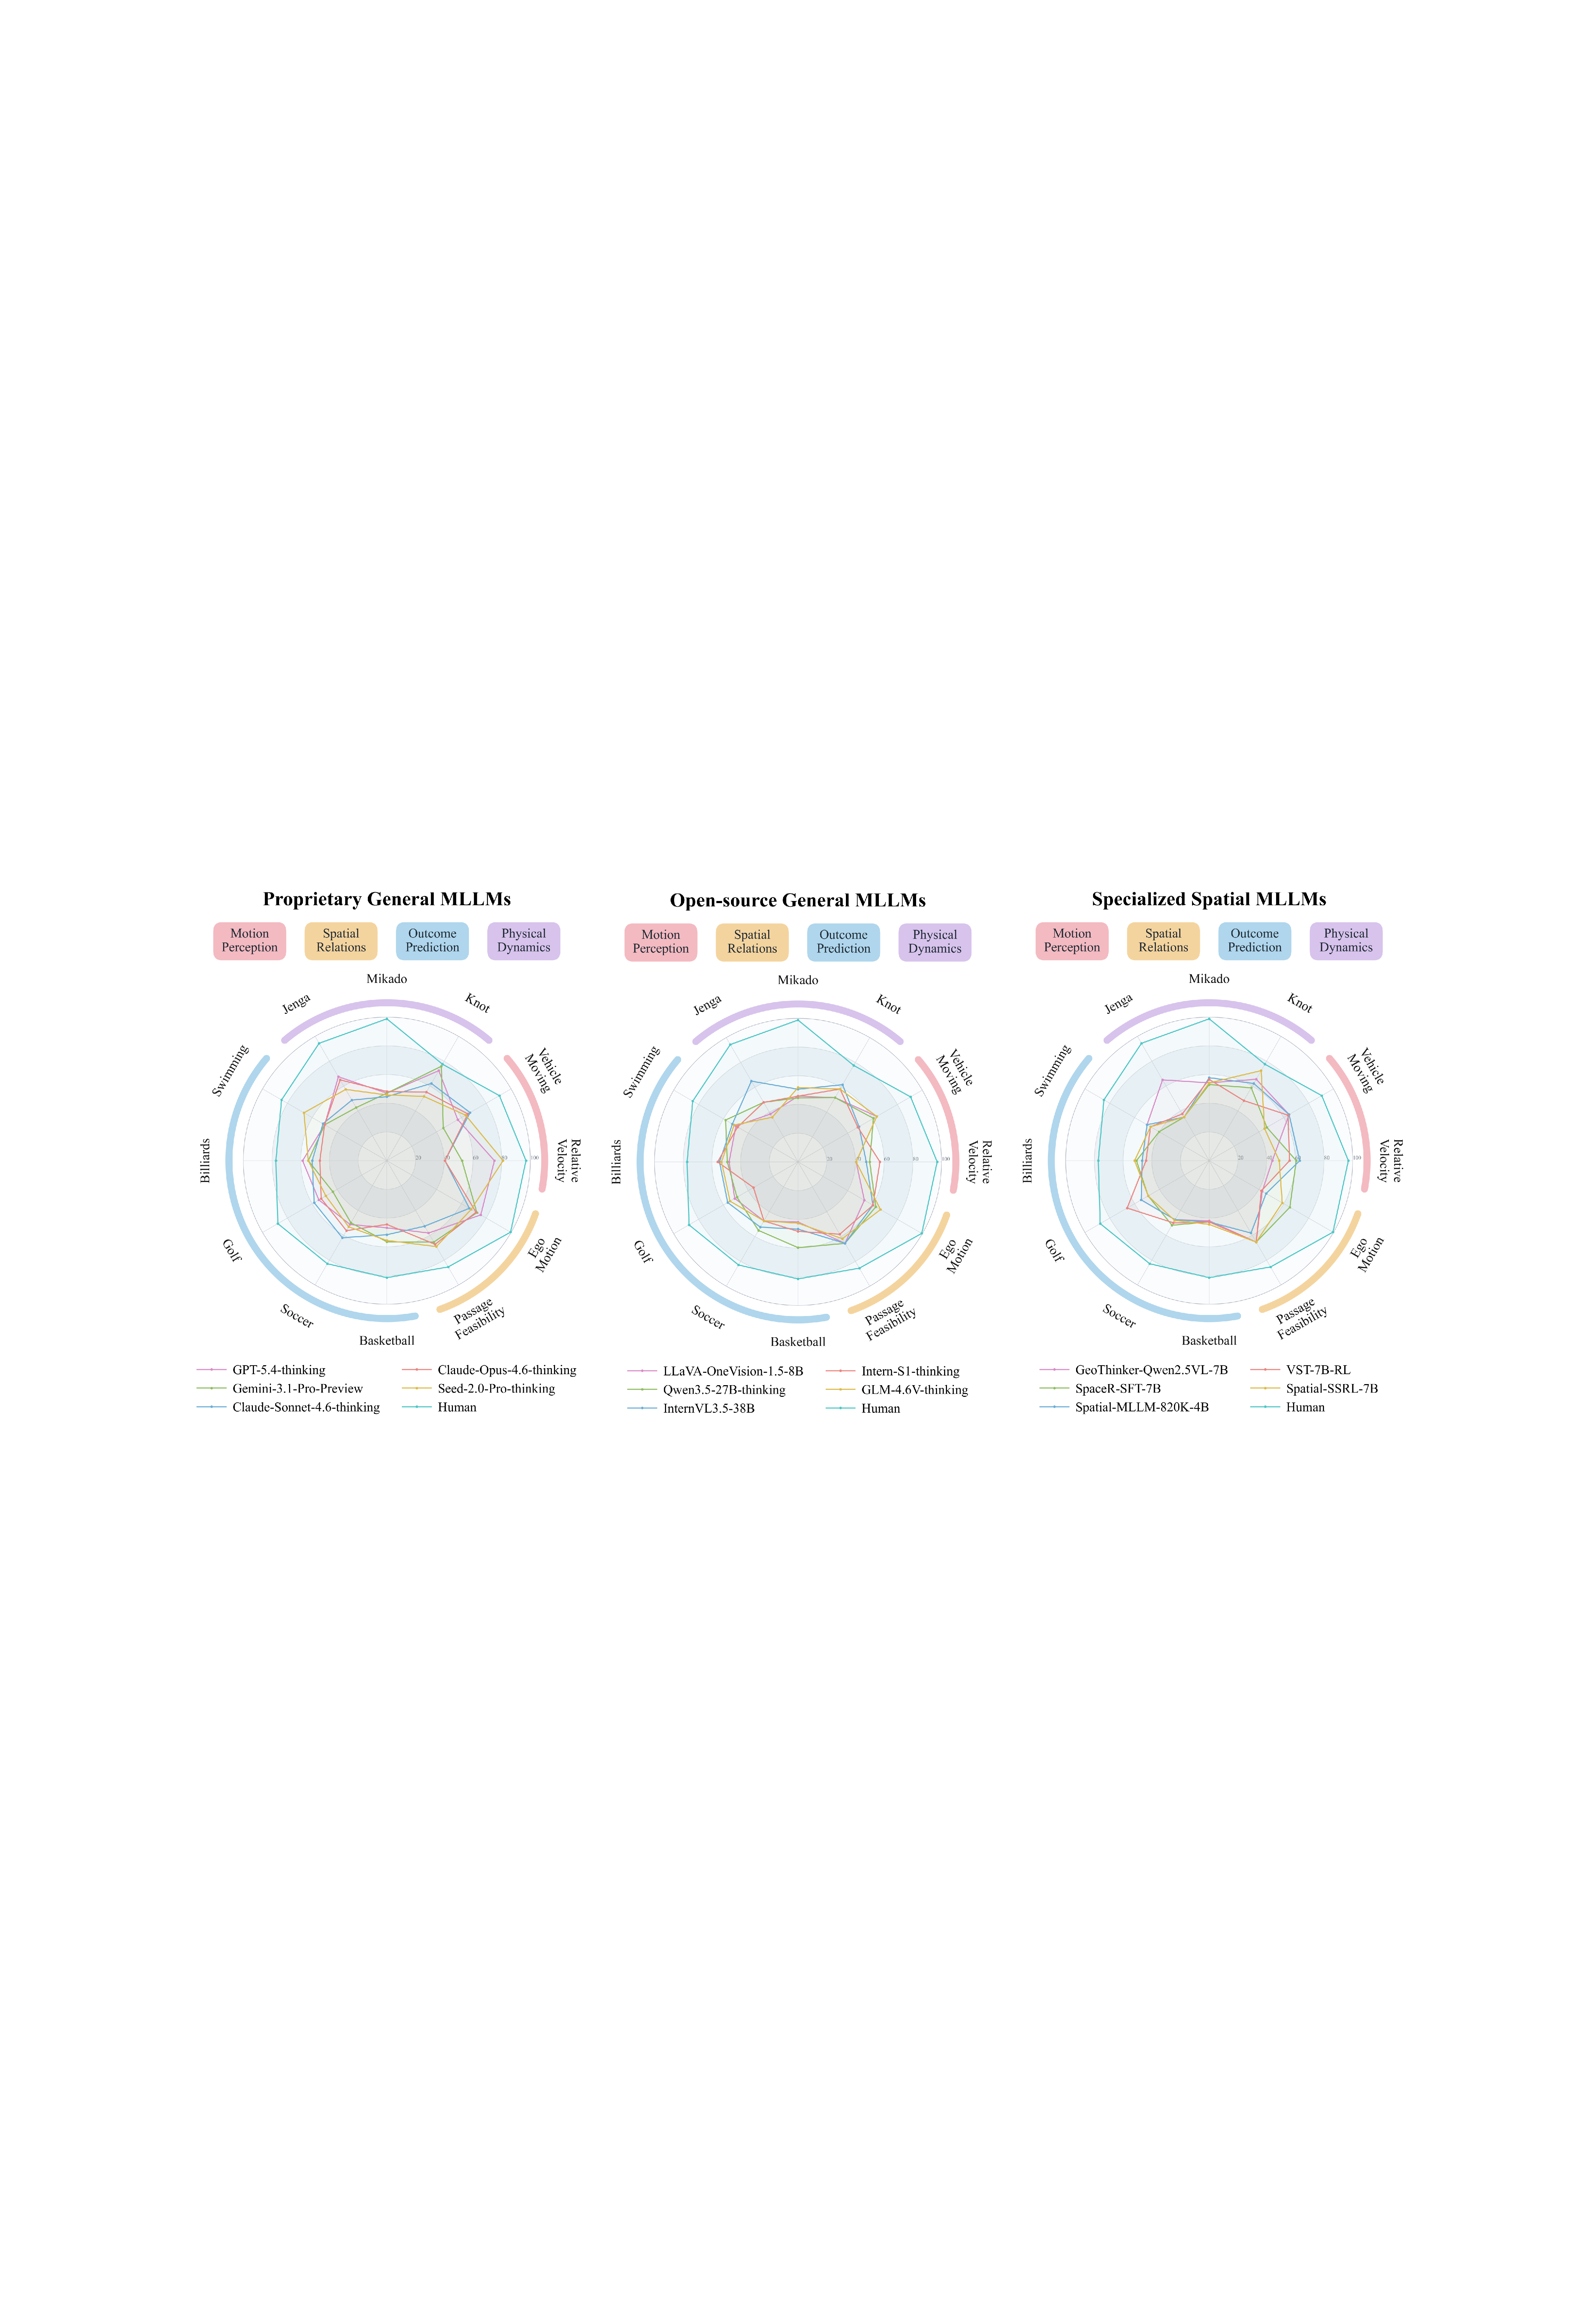
\includegraphics[width=0.9\linewidth]{fig/fig_5.pdf}
  \caption{\textbf{Radar comparison across model groups.} We visualize representative models from proprietary general-purpose MLLMs, open-source general-purpose MLLMs, and specialized spatial MLLMs across the 12 subtasks in ViSTR-Bench. Human performance is shown as a reference, highlighting the substantial gap between current MLLMs and human-level spatial-temporal reasoning.}
  \label{fig:5}
\end{figure}

\subsection{Main Results}
\label{sec:main_results}

Table~\ref{tab:main_results} and Figure~\ref{fig:5} report the comprehensive evaluation results on ViSTR-Bench. We summarize the main observations as follows.

\textbf{Current MLLMs remain far from human-level spatial-temporal reasoning.}
Existing MLLMs achieve limited performance on ViSTR-Bench.
The best-performing model, Seed-2.0-Pro-thinking, obtains an overall accuracy of 59.8\%, only 2.6\% higher than Chance Level (Frequency) and substantially below human performance of 89.0\%.
This large gap indicates that qualitative spatial-temporal reasoning from continuous visual cues remains a challenging problem for current MLLMs.
Moreover, the small margin over the frequency-based baseline suggests that many models still fail to reliably exploit dynamic visual evidence beyond dataset-level answer priors.

\textbf{Proprietary general-purpose MLLMs perform best overall.}
Among all evaluated model groups, proprietary general-purpose MLLMs achieve the best overall results.
Seed-2.0-Pro-thinking and Seed-2.0-Lite-thinking rank first and second, with accuracies of 59.8\% and 59.7\%, respectively, followed by GPT-5.4-thinking at 59.0\% and Claude-Opus-4.6 at 57.0\%.
In contrast, open-source general-purpose MLLMs generally obtain lower performance, with most models falling between 48\% and 55\%.
Notably, within the open-source families, relatively smaller dense models tend to outperform their larger Mixture-of-Experts counterparts.
For instance, Qwen3.5-27B-thinking achieves 55.1\%, surpassing the much larger Qwen3.5-397B-A17B-thinking at 54.3\%.
Similarly, InternVL3.5-38B achieves 54.5\%, outperforming InternVL3.5-241B-A28B at 54.1\%.
This suggests that, for complex continuous visual reasoning tasks, dense activation may provide more stable and reliable temporal representations than sparse routing mechanisms.

\textbf{Spatial MLLMs show limited generalization to dynamic reasoning.}
Although specialized spatial MLLMs are designed to enhance spatial intelligence, they do not show clear advantages on ViSTR-Bench.
The best model in this group, GeoThinker-Qwen2.5VL-7B, achieves only 52.0\% overall accuracy, which is close to random chance and lower than many general-purpose MLLMs.
Moreover, we observe that several specialized spatial MLLMs exhibit biased single-option prediction patterns on certain tasks.
As a result, their performance often matches Chance Level (Frequency) or its complementary value.
This suggests that spatial capability learned from static or geometry-centric training datasets~\citep{SPAR-Bench,LLaVA-Video} does not directly transfer to dynamic spatial-temporal reasoning.
ViSTR-Bench requires models to aggregate temporal evidence, track state changes, and reason about future outcomes or physical interactions, which remain weakly captured by current spatial MLLMs.

\textbf{Thinking mode is helpful but not consistently reliable.}
For models that support built-in thinking modes, enabling thinking often improves overall performance.
For example, GPT-5.4 improves from 54.9\% to 59.0\%, and Seed-2.0-Pro improves from 56.6\% to 59.8\%.
However, the improvement is not universal.
Claude-Opus-4.6 slightly drops from 57.0\% to 56.1\% after enabling thinking, and the gains for MiMo-V2.5 are marginal.
This indicates that explicit reasoning mechanisms can benefit spatial-temporal reasoning, but current thinking modes are not consistently beneficial across models.

\textbf{Performance varies substantially across reasoning dimensions.}
Models generally perform better on Motion Perception and Spatial Relations, where several top models achieve accuracies above 65\% on individual subtasks.
In contrast, Outcome Prediction and Physical Dynamics remain more challenging, with many results close to chance level.
These tasks require anticipating future outcomes or reasoning about latent physical dependencies, rather than merely recognizing visible motion or spatial relations.
This capability imbalance suggests that current MLLMs are better at describing observed dynamics than at performing temporally grounded prediction and intuitive physical reasoning.

\begin{table}[!t]
    \centering
    \caption{
        \textbf{Effect of text-based CoT prompting on ViSTR-Bench.}
        We evaluate Gemini-3.1-Pro-Preview~\citep{Gemini} with \emph{Direct Prompting} and various text-based CoT prompting strategies.
        \emph{Avg.} denotes the overall accuracy (\%) averaged over all question-answer pairs, and $\Delta$ denotes the accuracy change relative to \emph{Direct Prompting}.
        The best and second-best results are highlighted with \bestcap{} and \secondcap{}, respectively.
    }
    \label{tab:text_cot}

    \resizebox{\textwidth}{!}{
    \begin{tabular}{l c c cc cc ccccc ccc}
        \toprule
        \multirow{2}{*}{\textbf{Method}} 
        & \multirow{2}{*}{\textbf{Avg.}} 
        & \multirow{2}{*}{$\boldsymbol{\Delta}$} 
        & \multicolumn{2}{c}{\textbf{Motion Perc.}} 
        & \multicolumn{2}{c}{\textbf{Spat. Rela.}} 
        & \multicolumn{5}{c}{\textbf{Outc. Pred.}}  
        & \multicolumn{3}{c}{\textbf{Phys. Dyna.}} \\
        \cmidrule(lr){4-5} \cmidrule(lr){6-7} \cmidrule(lr){8-12} \cmidrule(lr){13-15}
        & & 
        & \makecell{Vehi.\\Move.} & \makecell{Rela.\\Velo.} 
        & \makecell{Ego\\Motion} & \makecell{Pass.\\Feas.} 
        & Bask. & Soccer & Golf & Bill. & Swim.
        & Jenga & Mikado & Knot \\
        \midrule

        \rowcolor{groupbg}
        \multicolumn{15}{l}{\textbf{Gemini-3.1-Pro-Preview}} \\
        Direct Prompting & 53.6 & - & \best{45.5} & 52.4 & 72.5 & \best{65.5} & \second{56.5} & 50.0 & 43.4 & \best{54.7} & 50.0 & 42.7 & 47.0 & \best{75.9} \\
        Zero-shot CoT & 53.3 & -0.3 & \second{41.1} & \second{56.0} & \second{74.0} & 58.2 & \best{57.3} & 52.5 & \second{50.9} & \second{46.7} & 48.6 & 42.7 & \second{49.4} & 65.5 \\
        Self-Consistency & \second{54.2} & \second{+0.6} & \second{41.1} & 52.4 & \second{74.0} & \second{63.6} & 55.6 & \second{53.2} & 47.2 & \second{46.7} & \second{56.9} & 47.9 & 48.2 & 69.0 \\
        Plan-and-Solve & \second{54.2} & \second{+0.6} & \best{45.5} & 50.0 & \best{76.3} & 61.8 & 54.0 & 51.3 & 49.1 & 44.0 & 45.8 & \second{53.8} & \best{50.6} & 69.0 \\
        Manual CoT & \best{56.0} & \best{+2.4} & \best{45.5} & \best{59.5} & 69.5 & 61.8 & 54.0 & \best{55.1} & \best{58.5} & 41.3 & \best{58.3} & \best{55.6} & \best{50.6} & \second{72.4} \\
        \bottomrule
    \end{tabular}
    }
\end{table}

\subsection{Effect of Text-based CoT Prompting}
\label{sec:text_cot}

We further investigate whether explicit text-based Chain-of-Thought (CoT) prompting can enhance spatial-temporal reasoning on ViSTR-Bench.
Using Gemini-3.1-Pro-Preview as a representative video-based MLLM, we compare four text-based CoT prompting strategies against Direct Prompting, namely Zero-shot CoT~\citep{zero-shot-cot}, Self-Consistency~\citep{self-consistency-coT}, Plan-and-Solve~\citep{plan-and-solve}, and Manual CoT inspired by OmniSpatial~\citep{OmniSpatial}.
Specifically, Zero-shot CoT appends a generic step-by-step reasoning instruction without task-specific design.
Self-Consistency samples multiple reasoning paths by running the Zero-shot CoT prompt over five independent trials and aggregates the final predictions via majority voting.
Plan-and-Solve instructs the model to first formulate a reasoning plan and then execute it to solve the problem.
Manual CoT decomposes each task into human-crafted, task-specific analysis steps tailored to its underlying spatial-temporal reasoning requirement. 
Detailed prompt templates for Manual CoT are provided in Appendix~\ref{sec:detailed_prompt_templates}.

As reported in Table~\ref{tab:text_cot}, text-based CoT prompting brings only limited and strategy-dependent improvements on ViSTR-Bench.
Zero-shot CoT slightly decreases the overall accuracy from 53.6\% to 53.3\% compared with Direct Prompting, suggesting that simply eliciting generic step-by-step reasoning is insufficient for complex video-based spatial-temporal reasoning.
Self-Consistency and Plan-and-Solve both improve the overall accuracy by 0.6\%.
This suggests that aggregating multiple reasoning paths or imposing a more structured reasoning process can help the model to some extent, but the gains remain marginal.
Manual CoT achieves the best overall performance, improving Direct Prompting by 2.4\% and reaching 56.0\%.
By decomposing each task into task-specific reasoning steps, Manual CoT provides stronger guidance for grounding textual reasoning in relevant visual evidence.
Nevertheless, the improvement is still moderate and highly task-dependent.
Moreover, even the best CoT result remains close to the chance-level baselines, indicating that text-based reasoning prompts alone cannot fully compensate for the limitations of current MLLMs in accurate visual perception and temporal grounding.

\begin{table}[!t]
    \centering
    \caption{
        \textbf{Effect of visual input format on ViSTR-Bench.}
        We evaluate Gemini-3.1-Pro-Preview~\citep{Gemini} with different visual input formats.
        \emph{Avg.} denotes the overall accuracy (\%) averaged over all question-answer pairs, and $\Delta$ denotes the accuracy change relative to \emph{Text-only}.
        The best and second-best results are highlighted with \bestcap{} and \secondcap{}, respectively.
    }
    \label{tab:visual_input}

    \resizebox{\textwidth}{!}{
    \begin{tabular}{l c c cc cc ccccc ccc}
        \toprule
        \multirow{2}{*}{\textbf{Input Format}} 
        & \multirow{2}{*}{\textbf{Avg.}} 
        & \multirow{2}{*}{$\boldsymbol{\Delta}$} 
        & \multicolumn{2}{c}{\textbf{Motion Perc.}} 
        & \multicolumn{2}{c}{\textbf{Spat. Rela.}} 
        & \multicolumn{5}{c}{\textbf{Outc. Pred.}}  
        & \multicolumn{3}{c}{\textbf{Phys. Dyna.}} \\
        \cmidrule(lr){4-5} \cmidrule(lr){6-7} \cmidrule(lr){8-12} \cmidrule(lr){13-15}
        & & 
        & \makecell{Vehi.\\Move.} & \makecell{Rela.\\Velo.} 
        & \makecell{Ego\\Motion} & \makecell{Pass.\\Feas.} 
        & Bask. & Soccer & Golf & Bill. & Swim.
        & Jenga & Mikado & Knot \\
        \midrule

        \rowcolor{groupbg}
        \multicolumn{15}{l}{\textbf{Gemini-3.1-Pro-Preview}} \\
        Text-only & 46.4 & - & \second{47.3} & \second{51.2} & 46.6 & 36.4 & 47.6 & 43.0 & \second{52.8} & \second{53.3} & 40.3 & 43.6 & 45.8 & 58.6 \\
        Last Frame & 50.4 & +4.0 & \best{48.2} & 45.2 & 54.2 & 45.5 & \second{50.0} & \second{55.7} & 49.1 & 48.0 & \best{58.3} & \second{44.4} & 45.8 & 65.5 \\
        Shuffled Frames & \second{52.3} & \second{+5.9} & \best{48.2} & \second{51.2} & 60.3 & 56.4 & 49.2 & \best{56.3} & \best{62.3} & 42.7 & 48.6 & \second{44.4} & \best{50.6} & \second{72.4} \\
        Ordered Frames & 51.7 & +5.3 & 46.4 & 47.6 & \second{67.2} & \second{58.2} & 49.2 & 55.1 & 49.1 & \second{53.3} & 47.2 & \best{48.7} & 36.1 & 62.1 \\
        Original Video & \best{53.6} & \best{+7.2} & 45.5 & \best{52.4} & \best{72.5} & \best{65.5} & \best{56.5} & 50.0 & 43.4 & \best{54.7} & \second{50.0} & 42.7 & \second{47.0} & \best{75.9} \\
        \bottomrule
    \end{tabular}
    }
\end{table}

\subsection{Effect of Visual Input Format}
\label{sec:visual_input}

We further study how different visual input formats affect model performance on ViSTR-Bench.
Using Gemini-3.1-Pro-Preview as the evaluated model, we compare five input settings: text-only input, the last frame only, shuffled frames with disrupted temporal order, ordered frames uniformly sampled from the video, and the original video input.
As reported in Table~\ref{tab:visual_input}, all visual input formats consistently outperform the text-only setting, showing that visual evidence provides useful cues beyond language priors.
Multi-frame inputs bring larger gains, with ordered frames and shuffled frames improving over the last-frame setting by 1.3\% and 1.9\%, respectively, suggesting that the model can benefit from observing multiple visual states.
However, shuffled frames slightly outperform ordered frames in overall accuracy, indicating that the model does not reliably exploit the continuous temporal order among frames.
This suggests that current MLLMs may capture coarse temporal-related cues from multiple frames, but still struggle to reason over continuous visual dynamics.
Original video input achieves the best performance, reaching 53.6\% overall accuracy.
These results indicate that video input provides the most complete visual evidence, while effective reasoning from continuous visual cues remains challenging for current MLLMs.
